\documentclass{article}
\usepackage{CJKutf8, indentfirst, graphicx, subfigure}
\begin{document}
\begin{CJK}{UTF8}{bsmi}
\title{硬體設計與實驗 Lab3 Report}
\author{
104021219 鄭余玄
}
\date{}
\maketitle
\section{實做過程}
clock\_divider 基本上和老師上課講義的 block diagram 作法差不多,
不過我把長度用 p 參數化,
因此除以 $2^{26}$ 和 $2^{19}$ 的 clock 就只需要改變參數而已。

lab3.xdc 是用助教附的 Basys3\_Master.xdc 去修改,因此很快就能完成。

lab3\_1 我是用 FSM 分成四種狀態亮燈,
分別是左邊向左 (LL)、左邊向右 (LR)、右邊向右 (RR)、右邊向左 (RL)。
在每個狀態下,增加亮燈的方法是用 bitwise or 位移目前的燈號,
這樣會使得有亮燈的地方持續,而位移到的新位置也可以亮燈。
同理,要使得亮燈處減少是用 bitwise and 位移目前的燈號,
這樣會保留共同有亮燈的地方,並且使新位置不亮燈。
至於狀態轉換,需要判斷是否燈號已滿,或是燈號已空,
這樣就是完整的 FSM 狀態轉移了。

lab3\_2 基本上就只有改變到 lab3\_1 的 clock。
因為 clock\_divider 是用參數化的寫法,
所以很容易就有 clk26 和 clk19 兩種頻率的訊號,
再利用 clk\_sel 做 clock 訊號選擇,
就完成這個 lab 了。
\subsection{Block diagram}
\begin{figure*}[h]
\centering{
  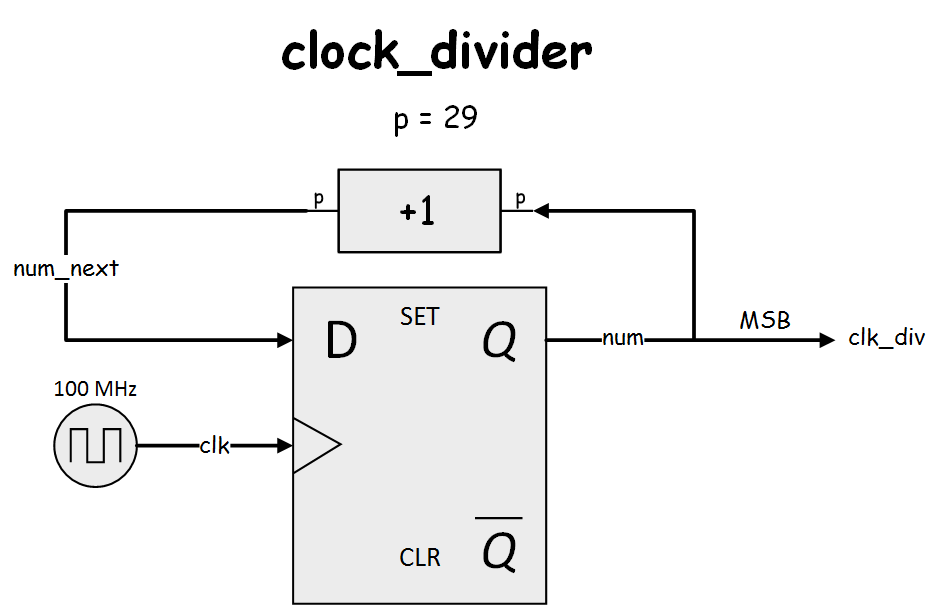
\includegraphics[width=.8\textwidth, angle=0]{clock_divider} \label{fig:cd}
}
\caption{clock\_divider}
\end{figure*}
基本上是參照老師的上課講義,不過我改用 p 去參數化。
\subsection{Finite State Machine}
\begin{figure*}[h]
\centering{
  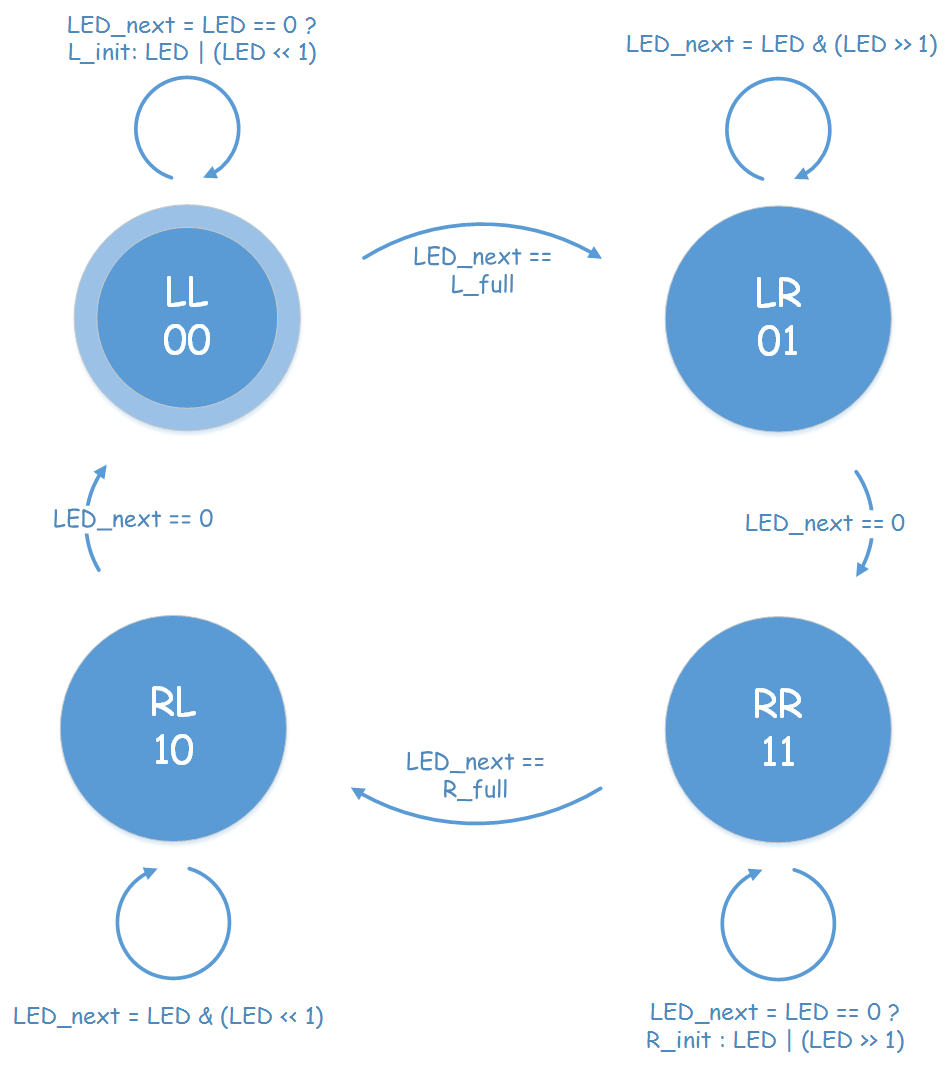
\includegraphics[width=1\textwidth, angle=0]{lab3_1} \label{fig:fsm}
}
\caption{lab3 FSM}
\end{figure*}
\section{心得}
這次的 lab 算是還滿順利的,
當老師講解完這次作業的時候,
基本上我已經想好如何實做了。
尤其是用 bitwise 亮燈的方法,
當初我是在想增加或減少亮燈,
就像是原本燈號做推移,
再疊加上原本的燈號,
因此我馬上就想出那個作法。

這次 lab 最麻煩的地方,
應該就是要 program 到 FPGA 上,
因為如果發現有一個小 bug,
就必須重新合成、實做、產生 bitstream,
最後才能跑在板子上。
所以這次學到最多的應該是先不要急著合成,
應該盡量確定沒有問題後再合成,
不然一等可能幾分鐘又過去了。

另外,這次的 report 我是用 Visio 去畫圖,
比起之前徒手畫工整許多,
也比較方便新增刪除狀態或物件。
\end{CJK}
\end{document}
